\chapter{Forecasting and Evaluation}
\label{chap:4}

The next step is to use the models constructed in the previous chapters for forecasting and to evaluate their performance. George E. P. Box is famously quoted as saying, \textit{“All models are wrong, but some are useful.”} In light of Box’s observation, the task now is to evaluate whether the models constructed are among those that are useful. The evaluation will proceed from two perspectives: a statistical perspective to assess model validity, and a risk management perspective to assess their practical usefulness.

To recap and introduce the forecasting procedure, the model parameters were estimated using S\&P 500 log returns from January 2014 to December 2024. The fitted models were then used to forecast the one-day-ahead variance and return density from January to April 2025. To assess their usefulness in a risk management context, the one-day-ahead Value at Risk (VaR) and Expected Shortfall (ES) are computed based on the forecasts from the fitted models.\footnote{Following standard risk-management convention, VaR and ES are reported as positive quantities representing the magnitude of a potential loss, even though the underlying returns in the loss tail are negative. This is why the formal definitions introduced later in the chapter carry a leading minus sign in front of the return quantile and tail expectation.}

As noted by \citeA{Christoffersen2012}, before using the variance model for forecasting, it is appropriate to subject the estimated model to diagnostic checks. In \hyperref[chap:1]{Chapter 1}, the dependence between squared returns was illustrated via the autocorrelation function (ACF) of squared returns. One of the primary objectives of volatility modeling is to eliminate this dependence structure by constructing a volatility measure, $\sigma^2_{t+1}$, such that the standardized squared returns, $\frac{R^2_{t+1}}{\sigma^2_{t+1}}$, exhibit no systematic autocorrelation patterns.

Figures~\ref{4.1} and~\ref{4.2} display the ACFs of the standardized squared returns (2014-2024) under the GARCH(1,1) and GJR-GARCH(1,1) models, respectively. It can be observed that the dependence structure seen in \hyperref[chap:1]{Chapter 1} has now disappeared, indicating that the GARCH models have been effective at removing the systematic autocorrelation patterns in the squared returns.

\begin{figure}[H]
    \centering
    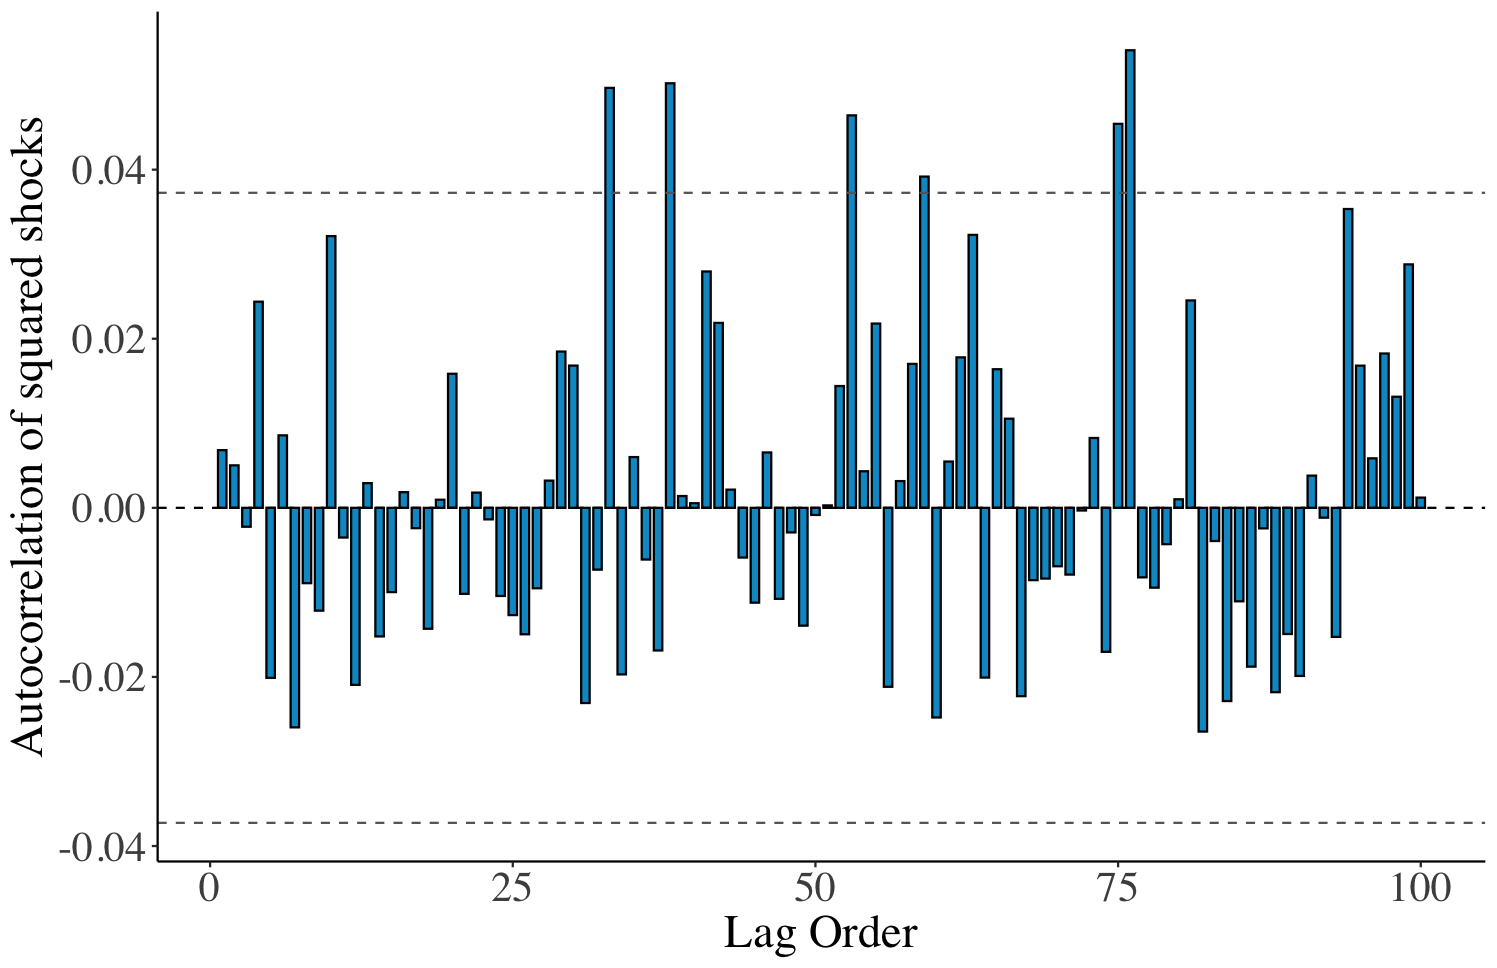
\includegraphics[scale=0.17]{../../plots/4.1.png} % Replace 
   \caption{Autocorrelation of squared returns over variance (2014-2024), GARCH(1,1).}
    \label{4.1}
\end{figure}

\begin{figure}[H]
    \centering
    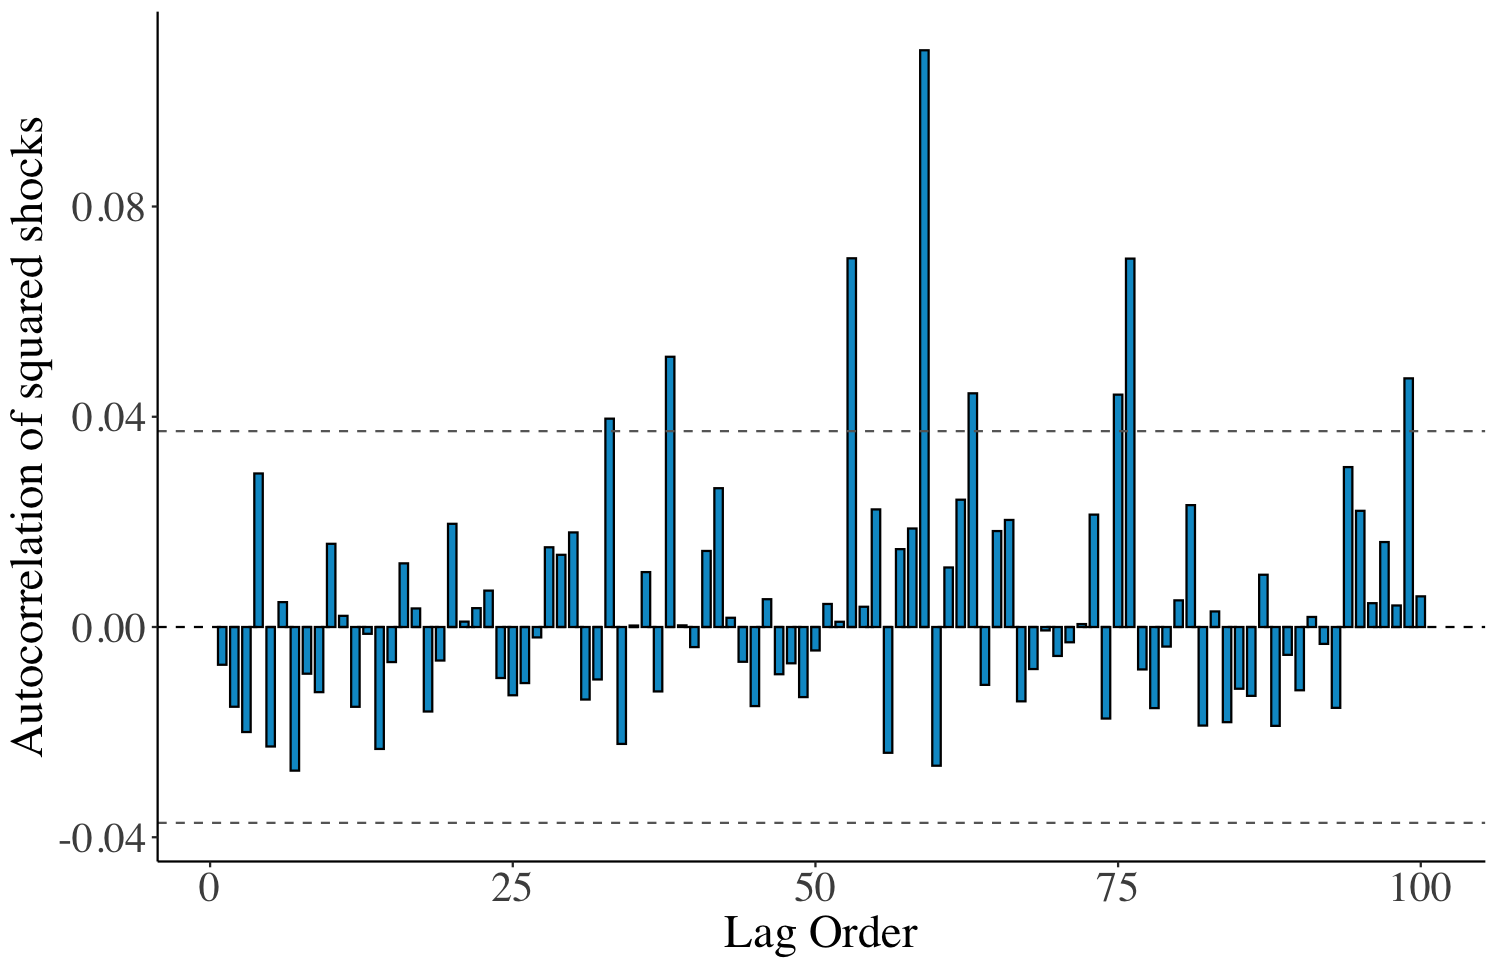
\includegraphics[scale=0.17]{../../plots/4.2.png} % Replace 
   \caption{Autocorrelation of squared returns over variance (2014-2024), GJR-GARCH(1,1).}
    \label{4.2}
\end{figure}

To complement the visual evidence, a Ljung–Box test was performed on the squared standardized residuals of both models using $m=7$ lags. The resulting $p$-values are 0.6528 for the GARCH(1,1) model and 0.3485 for the GJR-GARCH(1,1) model. In both cases, the null hypothesis that the first seven autocorrelations are jointly zero cannot be rejected. These results support the conclusion suggested by Figures~\ref{4.1} and~\ref{4.2}: the dependence structure originally present in squared returns has been effectively removed by the volatility models.

Before proceeding to forecasting, it is useful to assess which model performs better on the training set (2014–2024) under an appropriate loss function. When selecting a loss function, it is important to consider that risk managers may weigh positive and negative volatility forecast errors differently: underestimating volatility may be more costly than overestimating it by the same amount.

The QLIKE loss function addresses this asymmetry and is commonly used in the literature to evaluate volatility models, see \citeA{elliott201}. The QLIKE loss function is defined as:

\begin{equation}
\text{QLIKE}_t = \frac{R^2_{t+1}}{\sigma^2_{t+1}} - \ln\left(\frac{R^2_{t+1}}{\sigma^2_{t+1}}\right) - 1.
\label{eq:4.1}
\end{equation}

A loss function is said to be robust if the ranking of any two volatility forecasts is the same when using an observed volatility proxy as when (hypothetically) using the unobserved true volatility, as defined by \citeA{patton2011}. Robustness is clearly a desirable property for a volatility forecast loss function, and \citeA{patton2011} shows that the QLIKE loss function possesses this quality.

The mean QLIKE over the training period for both volatility models is reported in Table~\ref{tab:4.1}. The results suggest that the GJR-GARCH model outperforms the standard GARCH(1,1) model during the training period.

\begin{table}[htbp]
\centering
\begin{tabular}{lc}
\toprule
\textbf{Model} & Mean QLIKE \\
\midrule
GARCH(1,1)&  1.6011  \\
GJR-GARCH(1,1) & 1.5673 \\
\bottomrule
\end{tabular}
\caption{Mean QLIKE over the training period}
\label{tab:4.1}
\end{table}

The volatility models considered here were constructed using squared returns as the volatility proxy. As noted by \citeA{Christoffersen2012}, squared returns are an unbiased but potentially very noisy proxy for conditional variance. Alternatives include realized variance and range-based measures, which possess valuable predictive power and other desirable statistical properties. Readers interested in models based on alternative volatility proxies are referred to \citeA{Christoffersen2012} and the references therein. When using intraday-based proxies, it is important to account for market microstructure effects. \citeA{Tsay2010} and \citeA{Campbell1997} provide overviews of the microstructure of financial markets.

A simple likelihood ratio (LR) test can also be used to assess whether the additional parameter in the GJR-GARCH model is statistically significant relative to the simpler GARCH(1,1) model. As noted by \citeA{Christoffersen2012}, the LR test provides a straightforward way to evaluate whether added parameters are statistically meaningful.

Consider two nested models with log-likelihood values $L_0$ and $L_1$, where model 0 is a special case of model 1. The models can be compared using the likelihood ratio statistic:

\begin{equation}
\text{LR} = 2\left( \ln(L_1) - \ln(L_0) \right).
\label{eq:4.2}
\end{equation}

Under the null hypothesis that the additional parameter(s) in model 1 are not significant, the LR statistic follows a chi-squared distribution with degrees of freedom equal to the number of parameters added. In this case, since GJR-GARCH(1,1) adds one parameter to GARCH(1,1), the degrees of freedom equal 1.

Using the asymmetric $t$-distribution as the likelihood function, the LR test yields a $p$-value below 1\%, indicating little evidence in the data in favor of the null hypothesis. Thus, the additional parameter in the GJR-GARCH model is statistically significant.

Forecasting begins by considering the first two models in Table~\ref{tab:3.1}, which combine the volatility models with the asymmetric $t$-distribution. These models forecast the entire density of the next day’s return, allowing for the computation of risk measures such as Value-at-Risk (VaR) and Expected Shortfall (ES). Following the definition in \citeA{Christoffersen2012}, VaR is a risk measure that answers the question: What is the loss that will only be exceeded $p \times 100\%$ of the time on the next trading day? In other words, VaR corresponds to a quantile of the distribution of tomorrow’s return.

Under the specification $R_{t+1} = \sigma_{t+1} z_{t+1}$, with $z_{t+1} \sim \text{i.i.d. asyt}(d_1, d_2)$, the 1-day ahead $p$-level VaR can be computed as:
\begin{equation}
\text{VaR}_{t+1}^p = -\sigma_{t+1} \, F^{-1}_{\text{asyt}}(p; d_1, d_2),
\label{eq:4.3}
\end{equation}
where
\[
F^{-1}_{\text{asyt}}(p; d_1, d_2) =
\begin{cases}
\dfrac{1}{B} \left[(1 - d_2) \sqrt{\dfrac{d_1 - 2}{d_1}} \, t^{-1}_{p/(1 - d_2)}(d_1) - A \right], & \text{if } p < \dfrac{1 - d_2}{2} \\
\dfrac{1}{B} \left[(1 + d_2) \sqrt{\dfrac{d_1 - 2}{d_1}} \, t^{-1}_{(p + d_2)/(1 + d_2)}(d_1) - A \right], & \text{if } p \geq \dfrac{1 - d_2}{2}.
\end{cases}
\]
Here, $t^{-1}_{q}(d)$ denotes the $q$-th quantile of the symmetric Student's $t$-distribution with $d$ degrees of freedom.

The 1-day ahead Expected Shortfall (ES) is defined as
$$\text{ES}_{t+1}^p=-\mathbb{E}[R_{t+1}|R_{t+1}<-\text{VaR}_{t+1}^p],$$ 
and under the assumption of the asymmetric $t$-distribution, it can be computed as:
\begin{equation}
\text{ES}_{t+1}^p = -\sigma_{\text{PF}, t+1} \, \text{ES}_{\text{asyt}}(p),
\label{eq:4.4}
\end{equation}
where
\[
\begin{aligned}
\text{ES}_{\text{asyt}}(p) &= \dfrac{C(1 - d_2)^2}{Bp}
\left[1 + \dfrac{1}{d_1 - 2} \left(\dfrac{BQ + A}{1 - d_2}\right)^2 \right]^{\frac{1 - d_1}{2}} \dfrac{d_1 - 2}{1 - d_1} \\
&\quad - \dfrac{AC(1 - d_2)}{Bp} \cdot \dfrac{\sqrt{\pi(d_1 - 2)}\, \Gamma\left(\frac{d_1}{2}\right)}{\Gamma\left(\frac{d_1 + 1}{2}\right)} \, t_{d_1}\left(\sqrt{\dfrac{d_1}{d_1 - 2}} \cdot \dfrac{BQ + A}{1 - d_2}\right),
\end{aligned}
\]
and $Q=F^{-1}_{\text{asyt}}(p; d_1, d_2)$.

According to \citeA{elliott201}, a density forecast—such as those produced by combining volatility models with the asymmetric $t$-distribution—should satisfy certain desirable properties. One of these is \textit{calibration}, which requires that if a density forecast assigns a specific probability to an event, then the event should occur with approximately that frequency over successive observations.

This property can be assessed using Value-at-Risk. At the $p = 2.5\%$ level, a well-calibrated model should produce VaR breaches approximately 2.5\% of the time during the evaluation period. Figures~\ref{4.3} and~\ref{4.4} show the daily returns of the S\&P 500 from January to April 2025, along with the one-day-ahead 2.5\% VaR forecasts and the corresponding VaR breaches, assuming an asymmetric $t$-distribution.

With 81 observations in the test period, approximately two breaches would be expected under correct coverage. However, both models exhibit more than two breaches, indicating a failure to meet the calibration criterion. It is also worth noting the dynamic and adaptive behavior of the VaR forecast: following the market shock induced by Trump’s tariff imposition, volatility increased sharply. The VaR initially fails to capture this rise—resulting in several breaches—but gradually adjusts to the new, higher volatility regime. 

\begin{figure}[H]
    \centering
    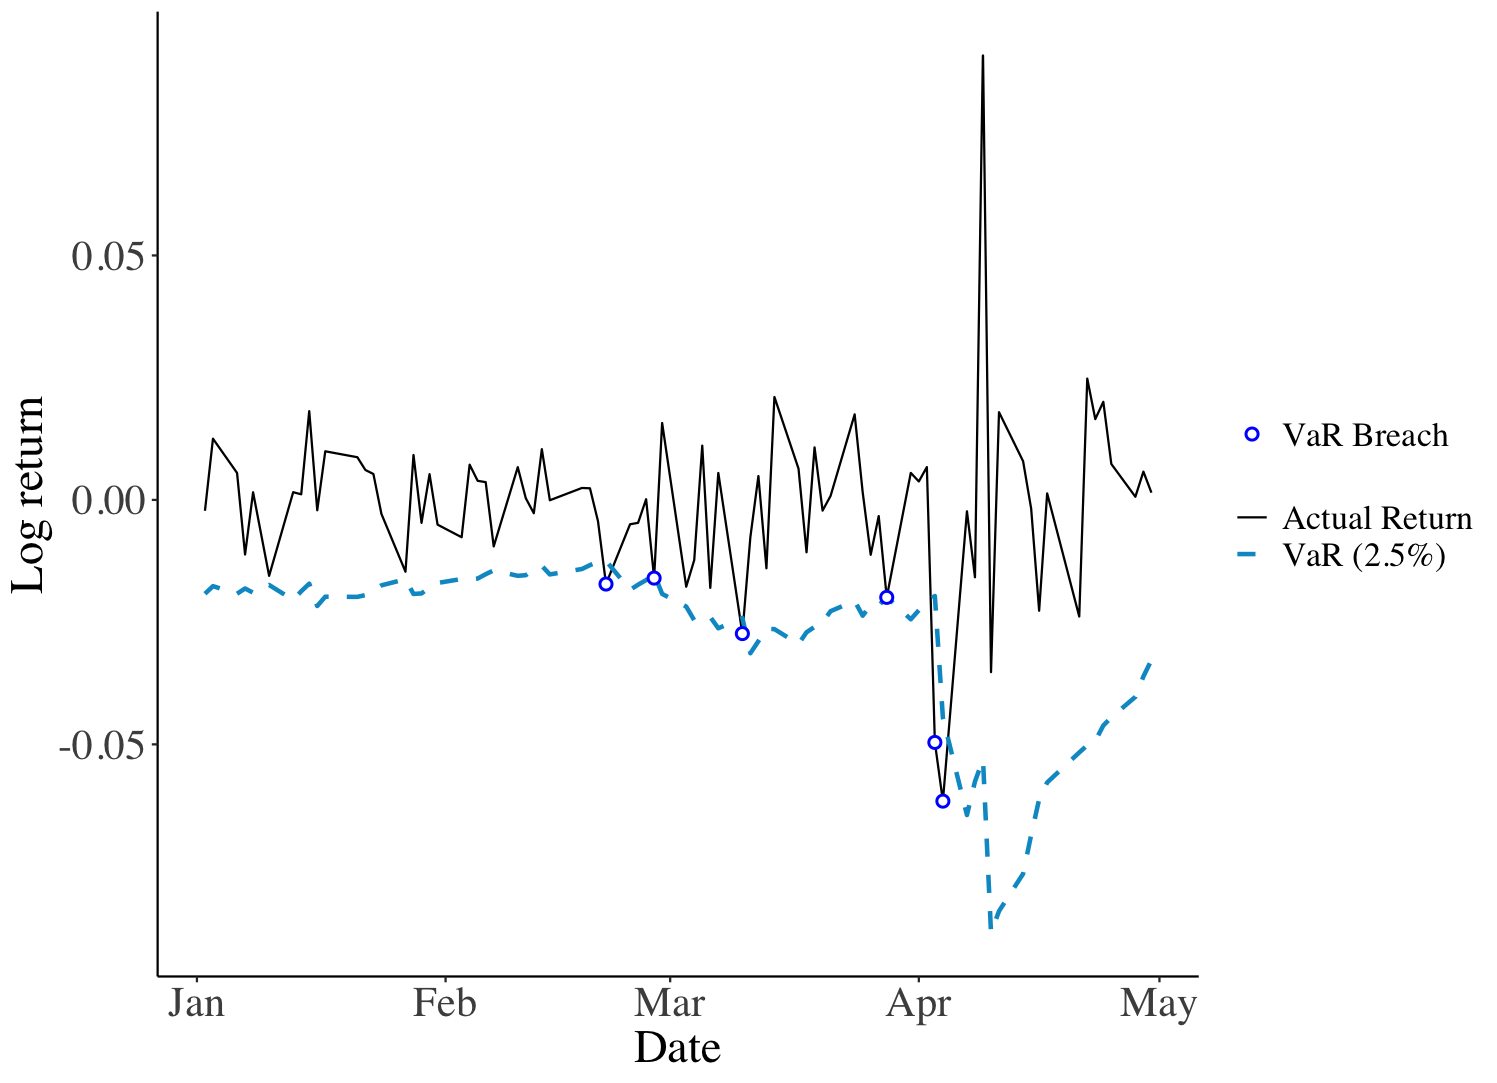
\includegraphics[scale=0.175]{../../plots/4.3.png} % Replace 
   \caption{2.5\% VaR forecast and breaches in the test period, GARCH-Asyt (6 breaches observed; 2 expected).}
    \label{4.3}
\end{figure}

\begin{figure}[H]
    \centering
    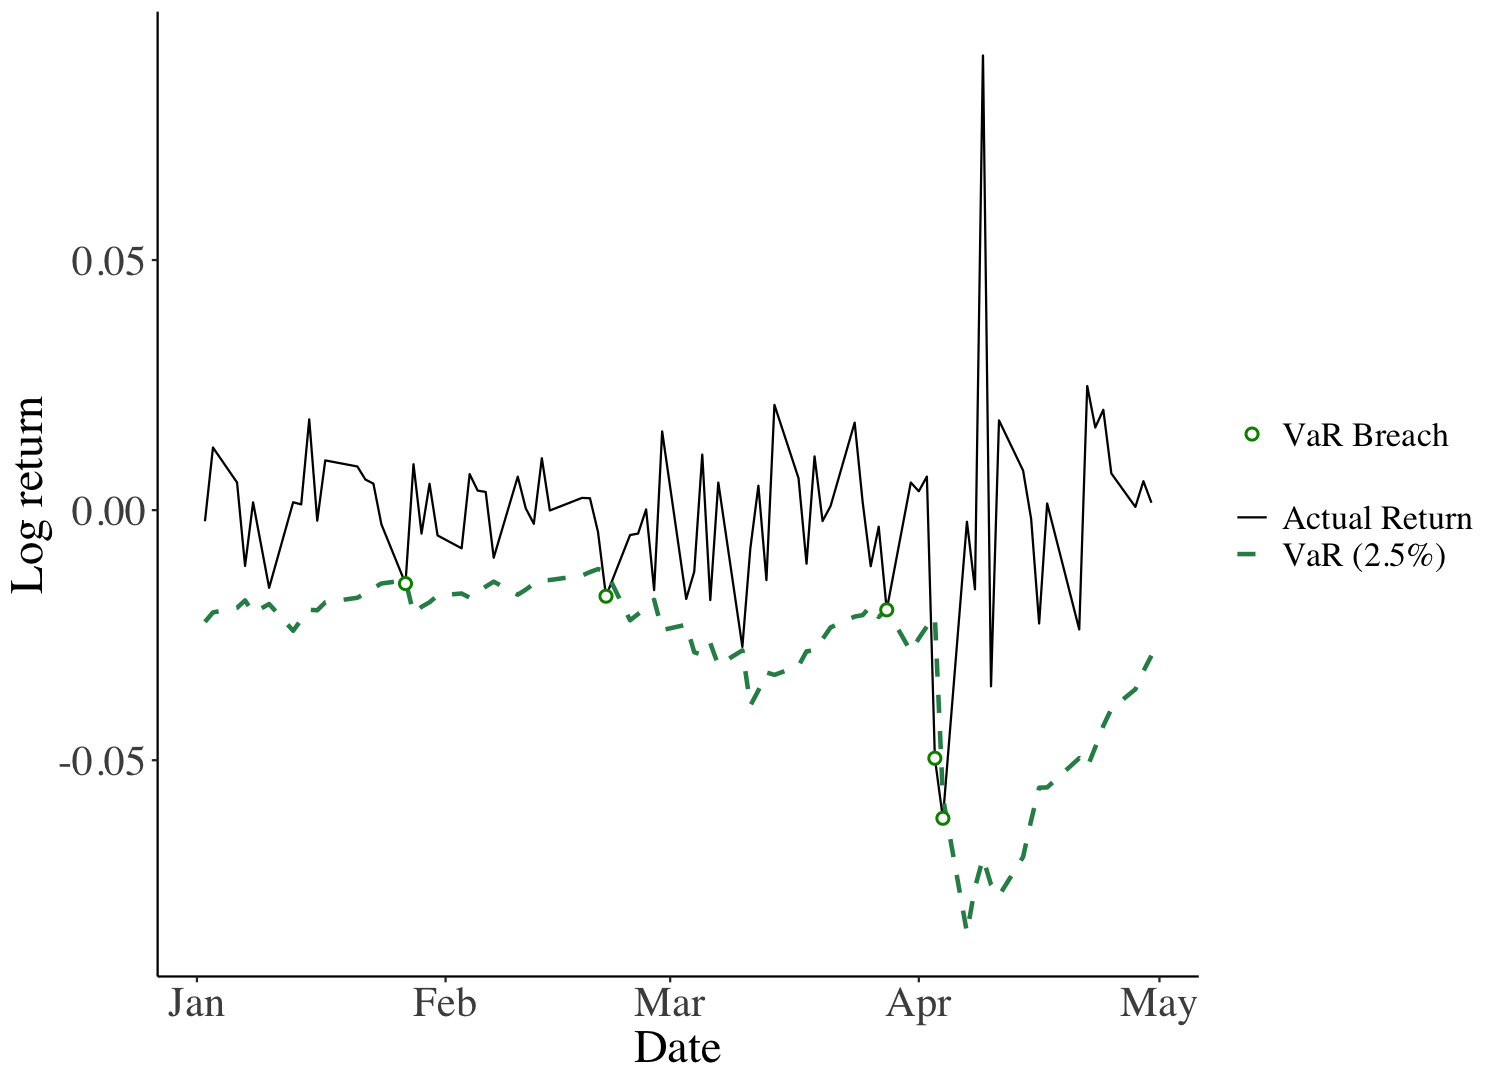
\includegraphics[scale=0.175]{../../plots/4.4.png} % Replace 
   \caption{2.5\% VaR forecast and breaches in the test period, GJR-Asyt (5 breaches observed; 2 expected).}
    \label{4.4}
\end{figure}

To improve the coverage of VaR and account for model risk, sources of uncertainty such as parameter estimation, model specification, and error distribution can be incorporated. \citeA{mazzeu2018uncertainty} propose several approaches to address these issues in ARMA models, which can be extended to the volatility models considered here.

As a simpler alternative, this chapter considers the use of Expected Shortfall (ES) as a way to stress the VaR forecast. Although ES is an expected value and does not correspond to a specific coverage level, it provides a more conservative risk measure by reflecting the average loss in the tail, thus functioning as a stressed version of VaR. Figures 4.5 and 4.6 display the 2.5\% Expected Shortfall for the previous models. It is worth noting that, among the cluster of consecutive breaches in early April in both Figures, only the first one also exceeds the ES forecast, illustrating how ES tempers the speed at which the conservative threshold is itself broken once volatility surges.

\begin{figure}[H]
    \centering
    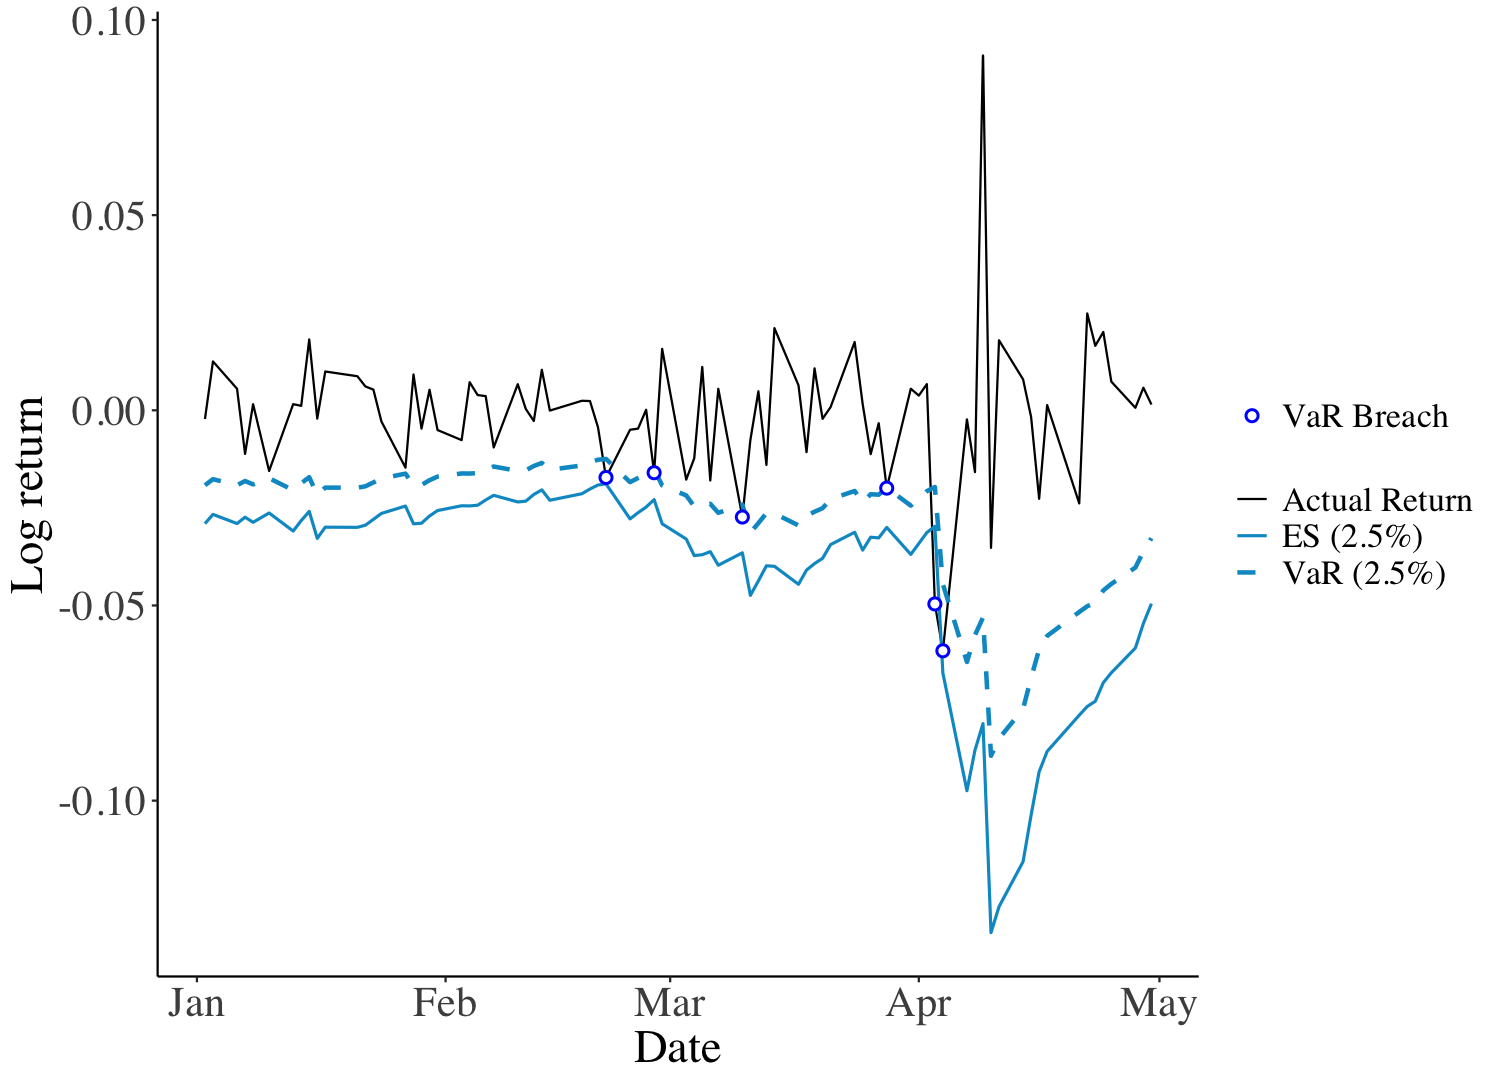
\includegraphics[scale=0.18]{../../plots/4.5.png} % Replace 
   \caption{2.5\% Expected Shortfall forecast in the test period,  GARCH-Asyt.}
    \label{4.5}
\end{figure}

\begin{figure}[H]
    \centering
    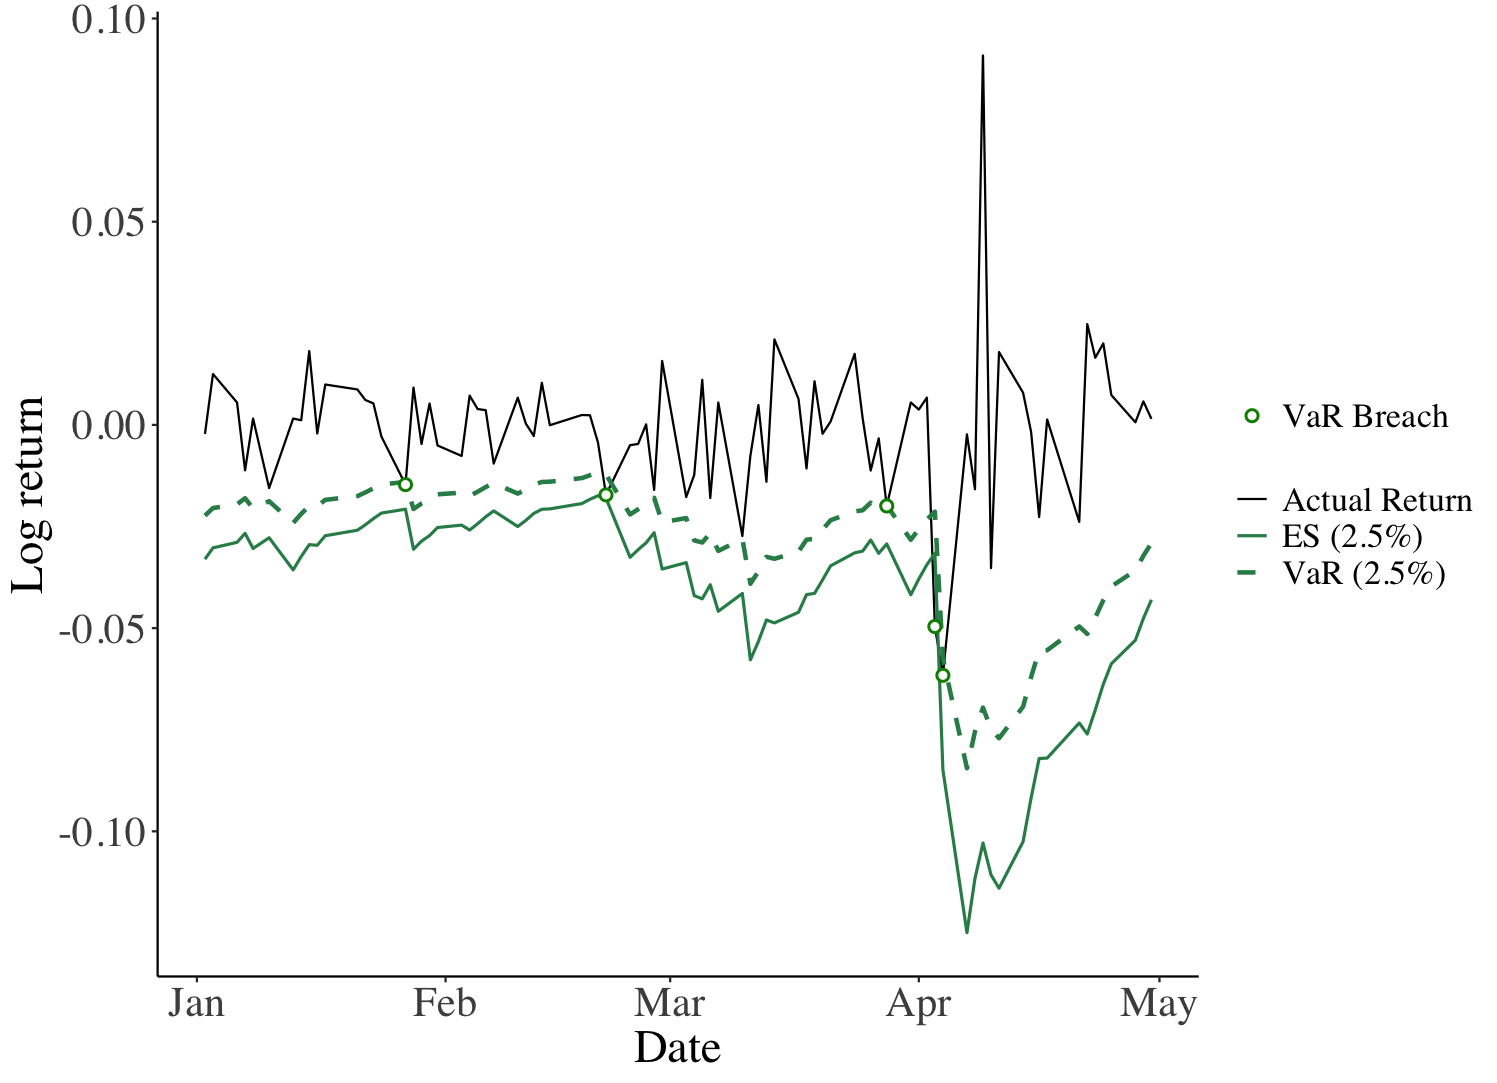
\includegraphics[scale=0.18]{../../plots/4.6.png} % Replace 
   \caption{2.5\% Expected Shortfall forecast in the test period,  GJR-Asyt.}
    \label{4.6}
\end{figure}

\citeA{christoffersen1998evaluating} provides an intuitive framework to evaluate the performance of VaR forecasts by testing two essential properties: coverage and independence.

Recall that a 1-day ahead VaR forecast at level $p$, denoted $\text{VaR}_{t + 1}^p$, implies that the actual return will fall below this threshold only $p \times 100\%$ of the time. Given a time series of ex-ante VaR forecasts and corresponding realized returns, the hit sequence of violations can be defined as follows:
\begin{equation}
I_{t+1} =
\begin{cases}
1, & \text{if } R_{t+1} < -\text{VaR}_{t+1}^p \\
0, & \text{if } R_{t+1} \geq -\text{VaR}_{t+1}^p.
\end{cases}
\label{eq:4.5}
\end{equation}

If the VaR model is correctly specified, violations should occur randomly with probability $p$ each day, implying that the hit sequence $\{I_{t+1}\}$ is independently and identically distributed (i.i.d.) as a $\text{Bernoulli}(p)$ random variable. Predictability of violations based on past information would indicate model misspecification and suggest room for improvement.

Three distinct properties can be tested, beginning with unconditional coverage. This test evaluates whether the observed frequency of breaches matches the expected frequency $p$. Let $\pi$ denote the parameter of the Bernoulli distribution governing the hit sequence, so that $I_{t+1}\sim \text{Bernoulli}(\pi)$. It can be estimated by
$\hat{\pi} = \frac{T_1}{T}$,
where $T_1$ is the number of violations observed in $T$ total observations. Since the Bernoulli likelihood is maximized at the sample mean, $\hat{\pi}=T_1/T$ is the maximum likelihood estimator of $\pi$. The hypotheses are then stated as
\[H_0:\pi=p \quad \text{vs.} \quad H_1:\pi\neq p.\]
The likelihood ratio test statistic for unconditional coverage is given by $LR_{\text{uc}} = -2 \ln\left( \frac{L(p)}{L(\hat{\pi})} \right)$ which, under the null hypothesis, asymptotically follows a $\chi^2$ distribution with 1 degree of freedom.\footnote{This result follows from the general asymptotic theory of likelihood ratio tests: under standard regularity conditions, the likelihood ratio statistic converges in distribution to a chi-squared random variable with degrees of freedom equal to the difference in the number of free parameters under the null and alternative hypotheses. See \citeA{casella2002statistical} for a standard treatment.}

Second, the independence of VaR violations can be assessed. Independence is critical; even if a VaR model achieves correct unconditional coverage, clustered violations would be problematic from a risk management perspective. Ideally, violations should occur randomly and independently, rather than grouping together in time. Therefore, testing for independence involves checking if the violations exhibit temporal clustering.

To conduct this test, assume the hit sequence $\{I_t\}$ follows a first-order Markov process characterized by the transition probability matrix:
\[
\Pi_1 =
\begin{bmatrix}
1 - \pi_{01} & \pi_{01} \\
1 - \pi_{11} & \pi_{11}
\end{bmatrix}.
\]
where, for example, the probability of a VaR violation tomorrow ($I_{t+1}=1$) given no violation today ($I_t=0$) is denoted by $\pi_{01}$. With a sample of $T$ observations, the likelihood function under this first-order Markov assumption is:
\[
L(\Pi_1) = (1 - \pi_{01})^{T_{00}} \, \pi_{01}^{T_{01}} \, (1 - \pi_{11})^{T_{10}} \, \pi_{11}^{T_{11}}.
\]
where $T_{ij}, \ i,j \in \{0,1\}$, is the number of times a state $j$ occurs immediately after state $i$.  The parameters $\pi_{01}$ and $\pi_{11}$ are estimated via maximum likelihood.

The null hypothesis of independence assumes that the probability of a violation does not depend on previous violations, thus simplifying the transition matrix to:
\[
\Pi_0 =
\begin{bmatrix}
1 - \pi & \pi \\
1 - \pi & \pi
\end{bmatrix}.
\]
The likelihood ratio test for independence and its distribution under the null hypothesis is:
\[
LR_{\text{ind}} = -2 \ln \left[ \dfrac{L(\hat{\Pi}_0)}{L(\hat{\Pi}_1)} \right] \dot\sim \chi^2_1,
\]
where $L(\hat{\Pi}_0)$ and $L(\hat{\Pi}_1)$ represent the maximum likelihood under the null hypothesis of independence and under the alternative hypothesis allowing dependence, respectively.

Lastly, it is critical to jointly test conditional coverage, evaluating simultaneously both independence and correct unconditional coverage. This is done via the conditional coverage likelihood ratio test which, under the null hypothesis, asymptotically follows a $\chi^2$ distribution with 2 degrees of freedom:
\[
LR_{\text{cc}} = -2 \ln \left[ \dfrac{L(p)}{L(\hat{\Pi}_1)} \right] \dot\sim \chi^2_2.
\]
which decomposes neatly into two previously described components:  $LR_{\text{cc}}=LR_{\text{uc}}+LR_{\text{ind}}$. 

In practice, backtesting frequently suffers from limited data, resulting in a relatively small number of violations $T_1$, which are crucial for the tests. Thus, relying on asymptotic $\chi^2$ distributions may not always be appropriate. Monte Carlo simulated $p$-values provide a robust alternative in this scenario. \citeA{christoffersen2004backtesting} discuss the implementation of such Monte Carlo-based $p$-values, a method originally proposed by Dufour in a 2000 manuscript that the authors cite and that was later published as \citeA{dufour2006monte}.

To calculate these simulated $p$-values, generate 999 random samples of $\text{i.i.d. Bernoulli}(p)$ variables, each of length $T$, matching the actual sample size. From these artificial samples, compute 999 simulated test statistics, denoted as $\{\widetilde{LR}_{\text{uc}}(i)\}_{i=1}^{999}$. Finally, the simulated $p$-value is calculated as the proportion of simulated $LR_{\text{uc}}$ statistics exceeding the observed test statistic, providing a reliable measure of the test’s significance.

Table~\ref{tab:4.2} reports the theoretical and simulated $p$-values for the tests proposed by \citeA{christoffersen1998evaluating}, applied to the GARCH-Asyt and GJR-Asyt models.

\begin{table}[H]
\centering
\begin{tabular}{llcc}
\toprule
\textbf{Test} & \textbf{p-value} & \textbf{GARCH-Asyt} & \textbf{GJR-Asyt} \\
\midrule
$LR_{\text{uc}}$   & Theoretical & 0.0215 & 0.0735 \\
                   & Simulated   & 0.003 & 0.144 \\
$LR_{\text{ind}}$  & Theoretical & 0.4332 & 0.2793 \\
                   & Simulated   & 0.095 &  0.047 \\
$LR_{\text{cc}}$   & Theoretical & 0.0523 & 0.1123 \\
                   & Simulated   & 0.015 & 0.028 \\
\bottomrule
\end{tabular}
\caption{Theoretical and simulated $p$-values for VaR backtesting statistics.}
\label{tab:4.2}
\end{table}

These models exhibit weak performance: they fail to achieve acceptable coverage, and the violations do not seem independent. As shown in Figures~\ref{4.3} and~\ref{4.4}, two breaches occur in quick succession at the onset of President Trump’s tariff imposition, indicating slow adaptation to a sharp increase in volatility and resulting in clustered VaR violations.

Attention now turns to evaluating the quality of the density forecasts. Focusing on the full forecasted return distribution offers the advantage of potentially increasing the power to reject misspecified risk models.

The GARCH-Asyt and GJR-Asyt models generate a one-step-ahead cumulative distribution forecast for the next day’s return, denoted $F_t(\cdot)$, at the end of each trading day. After observing the actual return $R_{t+1}$, the cumulative probability assigned to this outcome by the forecasted distribution can be evaluated. This probability, known as the Probability Integral Transform (PIT), was introduced by \citeA{diebold1998evaluating} and is defined as:
\begin{equation}
u_{t+1} = F_t(R_{t+1}).
\label{eq:4.6}
\end{equation}

\citeA{diebold1998evaluating} show that if the risk model used to forecast the return distribution is correctly specified, then the sequence $\{u_{t+1}\}$ should be independently and identically distributed as \text{Uniform}(0,1). Intuitively, this means that if the forecasted distribution is correct, the PIT values should not be predictable or systematically biased.

To assess the validity of the risk models considered here, the hypothesis of interest is:

\[H_0: u_{t+1} \sim \text{i.i.d. Uniform}(0,1).\]

\newpage
\citeA{diebold1998evaluating} suggest a visual diagnostic using a histogram of the PIT values $\{u_{t+1}\} $ to assess whether they appear approximately uniform. If systematic deviations from flatness are observed, this may indicate that the forecast distribution is misspecified. Figures~\ref{4.7} and~\ref{4.8} display the PIT histograms for the GARCH-Asyt and GJR-Asyt models over the test period, respectively. There are no evident deviations from uniformity.

\begin{figure}[H]
    \centering
    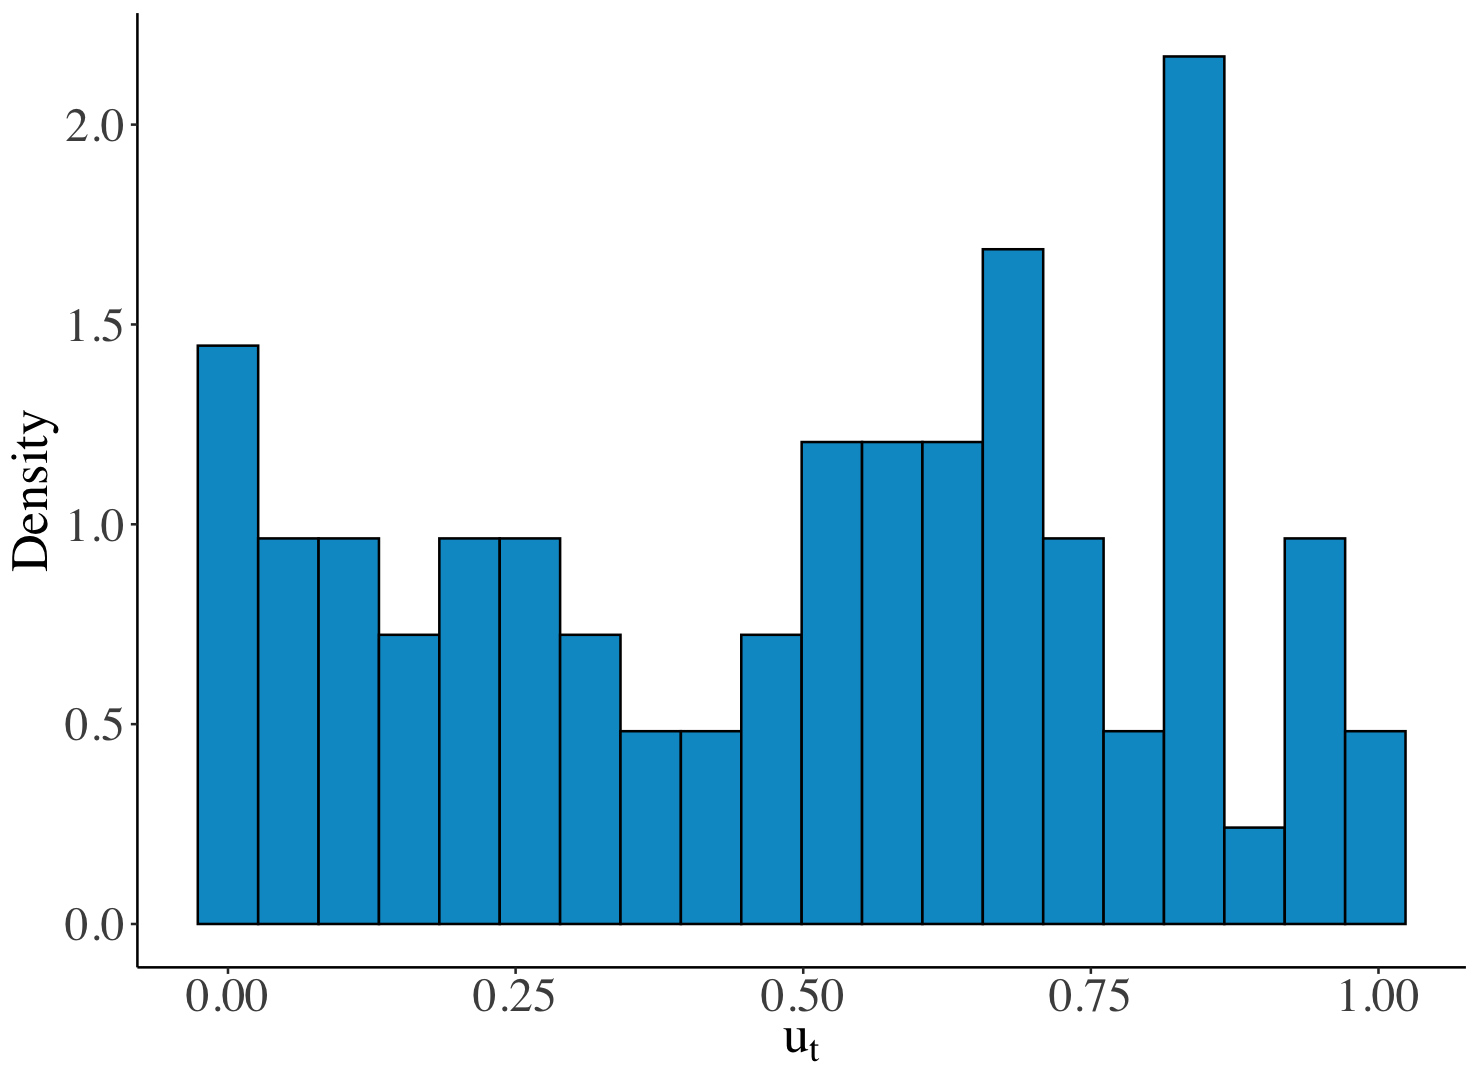
\includegraphics[scale=0.18]{../../plots/4.7.png} % Replace 
   \caption{ Histogram of PIT values, GARCH- Asyt.}
    \label{4.7}
\end{figure}

\begin{figure}[H]
    \centering
    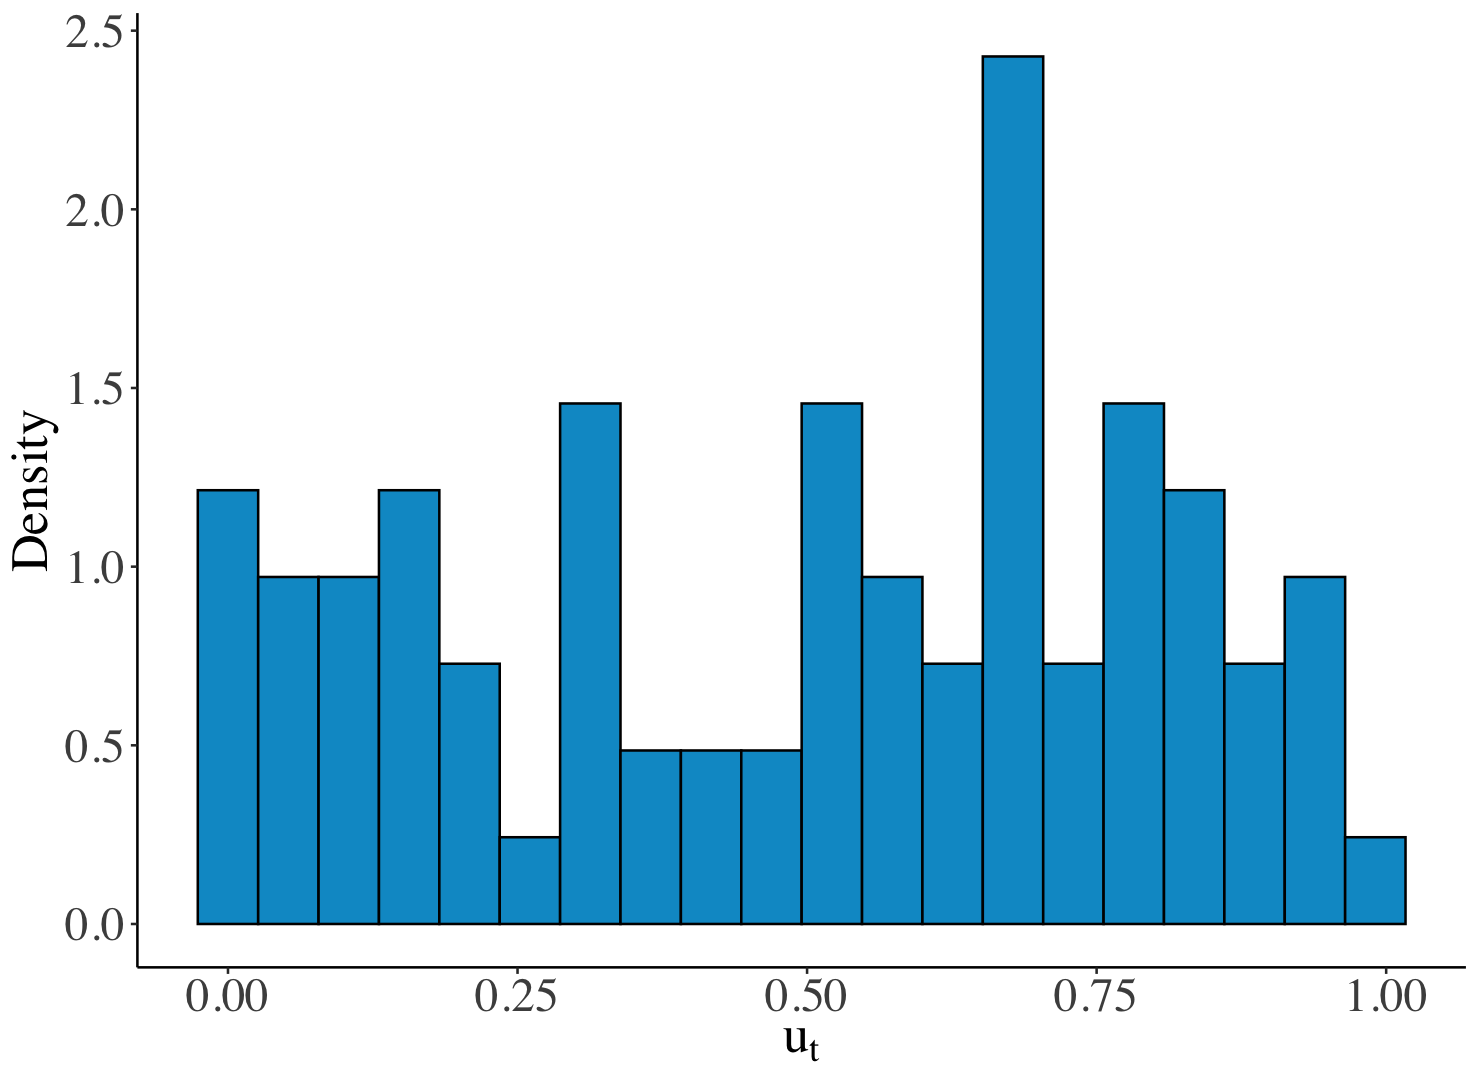
\includegraphics[scale=0.18]{../../plots/4.8.png} % Replace 
   \caption{ Histogram of PIT values, GJR- Asyt.}
    \label{4.8}
\end{figure}

While the histogram provides an intuitive diagnostic, it is not a formal statistical test. As noted by \citeA{Christoffersen2012}, testing the i.i.d. uniformity hypothesis is challenging due to the bounded support of the uniform distribution. To address this, \citeA{berkowitz2001testing} proposes transforming the PIT values to a standard normal scale and applying standard statistical tests to the transformed series:

\begin{equation}
\hat{z}_{t+1} = \Phi^{-1}(u_{t+1}),
\label{eq:4.7}
\end{equation}
where $\Phi^{-1}(\cdot)$ denotes the inverse of the standard normal cumulative distribution function. The hypothesis of interest becomes:

\[H_0: \hat{z}_{t+1} \sim \text{i.i.d. N}(0,1).\]

To test this hypothesis, a Kolmogorov–Smirnov (KS) test can be applied to the GARCH-Asyt and GJR-Asyt models to assess the validity of the density forecasts. Figures~\ref{4.9} and~\ref{4.8} display the empirical cumulative distribution functions of the transformed series $\{\hat{z}_{t+1}\}$ plotted against the standard normal CDF, with the KS test statistics indicated.

\begin{figure}[H]
    \centering
    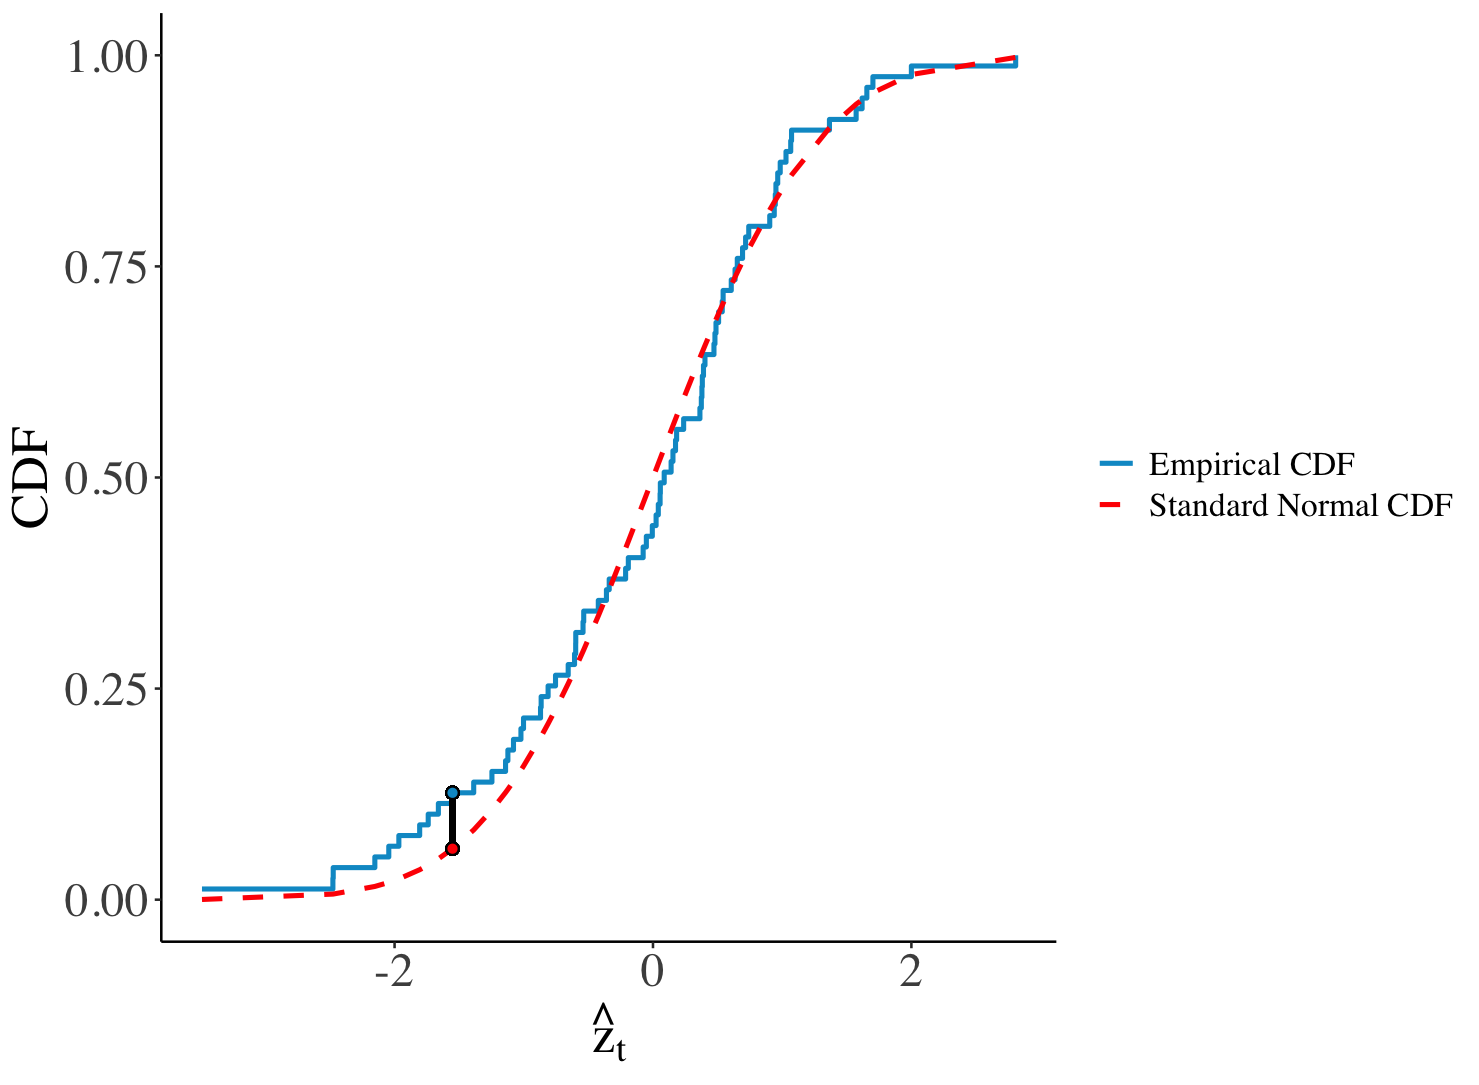
\includegraphics[scale=0.18]{../../plots/4.9.png} % Replace 
   \caption{Kolmogorov-Smirnov test on $\hat{z}_{t+1}$, GARCH-Asyt.}
    \label{4.9}
\end{figure}

\begin{figure}[H]
    \centering
    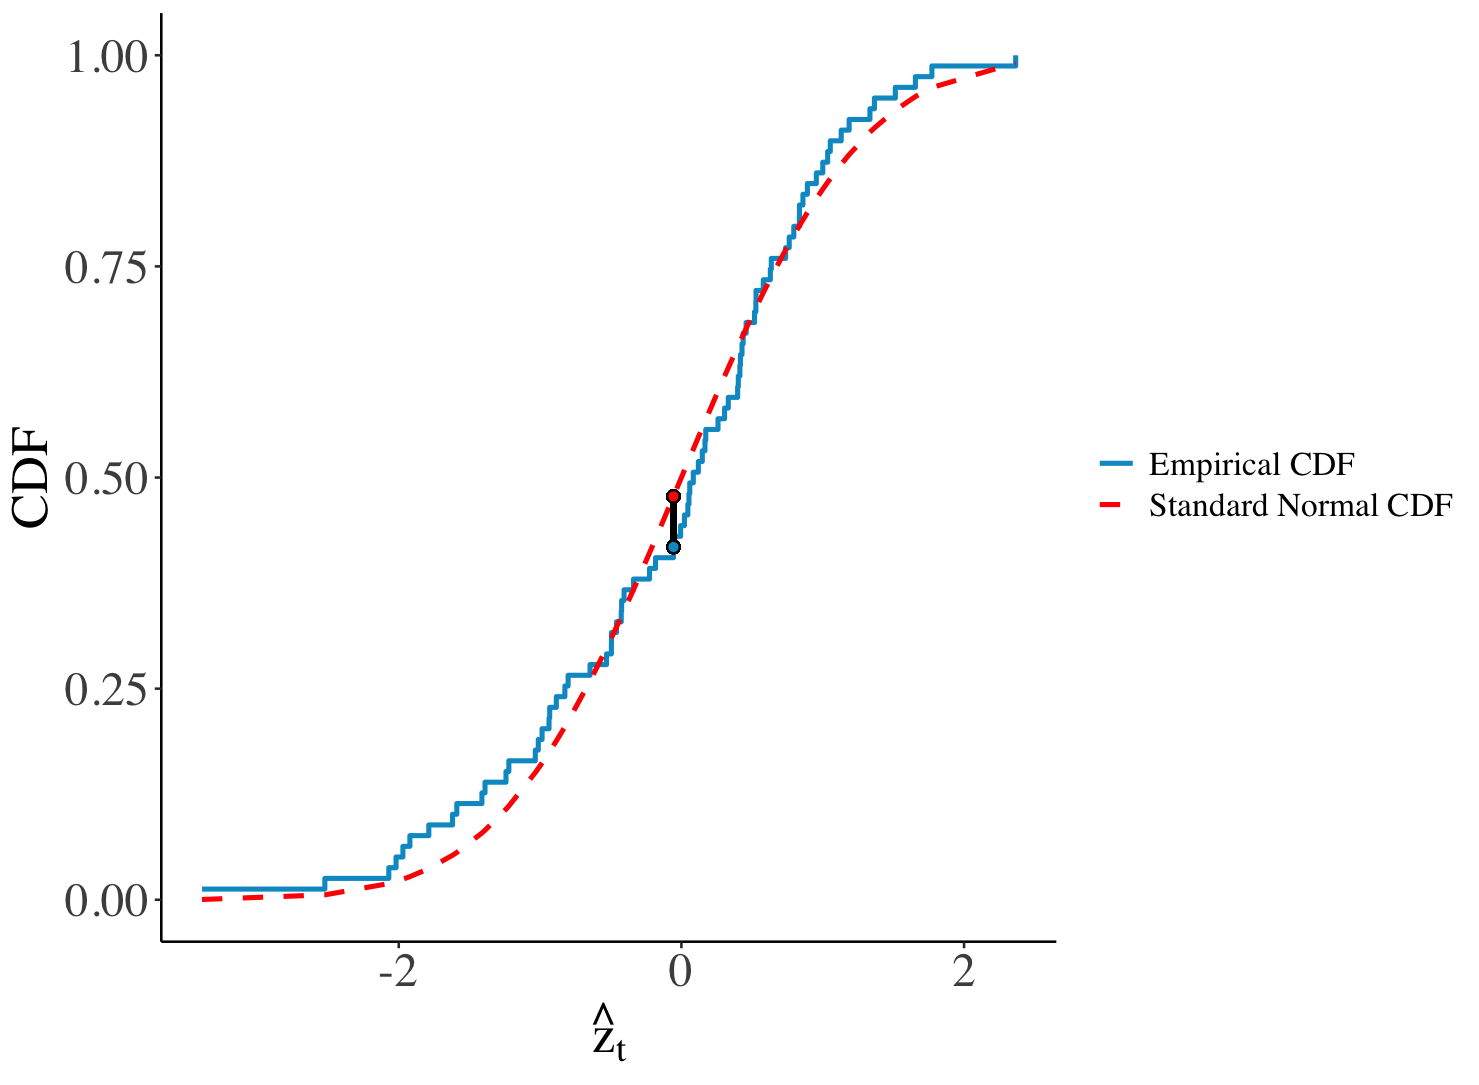
\includegraphics[scale=0.18]{../../plots/4.10.png} % Replace 
   \caption{Kolmogorov-Smirnov test on $\hat{z}_{t+1}$, GJR- Asyt.}
    \label{4.10}
\end{figure}

The resulting $p$-values for the GARCH-Asyt and GJR-Asyt models are 0.8512 and 0.7931, respectively. These values suggest that the hypothesis of normality cannot be rejected, supporting the validity of the models’ density forecasts. In addition, \citeA{berkowitz2001testing} proposes a likelihood ratio (LR) test to jointly assess normality and independence. Specifically, the hypothesis

\[H_0: \hat{z}_{t+1} \sim \text{i.i.d. N}(0,1) \quad vs.\quad H_1: \hat{z}_{t+1} \sim \text{N}(\hat{\mu},\hat{\sigma}^2) \] 

$\text{with autocorrelation }\rho$, can be tested via an LR statistic. The resulting $p$-values for the GARCH-Asyt and GJR-Asyt models are 0.3089 and 0.6577, respectively, indicating that the null hypothesis cannot be rejected.

To formally compare the density forecasts during the test period, the Diebold–Mariano (DM) test introduced by \citeA{diebold1995comparing} is employed. This test compares the accuracy of two competing forecast models under a specified loss function, which in this case is the negative log-likelihood function of the actual returns given the forecasted densities. Using the log-likelihood as a scoring rule follows the suggestion of \citeA{elliott201} for evaluating density forecasts. 

The DM test statistic is defined as:
\[
\text{DM} = \frac{\bar{d}}{\hat{\sigma}_d/\sqrt{T}},\]

where $\bar{d}$ is the average difference in log-likelihood scores, $d_t = \ell^{\text{(GARCH)}}(R_{t+1}|F_{t}) - \ell^{\text{(GJR)}}(R_{t+1}|F_{t})$,

with $\ell^{(m)}(\cdot)$ and $\ell^{(n)}(\cdot)$ representing the log-likelihoods of the two competing models. Here, $\hat{\sigma}_d$ denotes the standard deviation of the series $\{d_t\}$, and $T$ is the sample size. Under the null hypothesis of equal forecast accuracy, the DM statistic follows a standard normal distribution. 

After performing the test, the resulting $p$-value is 0.015, with a positive test statistic, suggesting that the GJR-Asyt density forecast provides significantly better forecasting performance compared to the GARCH-Asyt model. 

\citeA{corradi2006predictive} provide an extensive survey of methods to evaluate and compare density forecasts, both in-sample and out-of-sample. Readers interested in further methods for evaluating density forecasts are referred to this comprehensive survey. 

Attention now turns toward the GARCH-EVT and GJR-EVT models. These models provide conditional tail distributions rather than full-density forecasts. Informally, one might describe them as tail forecasts. Although several frameworks exist to evaluate tail forecasts, such as those proposed by \citeA{berkowitz2001testing} and \citeA{Christoffersen2012}, these approaches cannot be directly adapted to the conditional GARCH-EVT and GJR-EVT models considered here. Thus, these two models will only be assessed from a risk management perspective; a rigorous statistical validation method remains to be formally established. One possible validation strategy could involve adapting the PIT approach specifically for observations exceeding the threshold $u$, but this idea has not yet been fully explored in the reviewed literature.

According to the Pickands–Balkema–de Haan theorem, for sufficiently large threshold $u$,
\[
\frac{F(y) - F(u)}{1 - F(u)} \approx G_{u, \xi,\beta}(y) \quad \text{for } y>u,
\]

where $G_{u, \xi, \beta}(y)$ denotes the cumulative distribution function (CDF) of the generalized Pareto distribution (GPD). Approximating the CDF $F(u)$ of the standardized returns using the empirical distribution, we have:
\[
\hat{F}(u) = \frac{T - N_{u}}{T},
\]
where $N_u$ is the number of threshold exceedances and $T$ is the training sample size. Consequently, the tail distribution can be approximated by:
\[
F(y) \approx  F(u) + G(y)[1 - F(u)] \approx 1 - \frac{N_{u}}{T} \left[ 1 + \frac{\xi(y - u)}{\beta} \right]^{-1/\xi}.
\]
This approximation provides a direct method to estimate quantiles used for VaR calculations. Specifically, for a small tail probability $p$, letting $q = 1 - p$, solving the previous equation for $y$ yields the estimated VaR of the standardized returns:

\begin{equation}
    \text{VaR}_{z,t+1}^{p} =  u - \frac{\beta}{\xi} \left\{ 1 - \left[ \frac{T}{N_{u}} (1 - q) \right]^{-\xi} \right\}.
    \label{eq:4.8}
\end{equation}

Consequently, the VaR of actual returns is given by:
\begin{equation}
    \text{VaR}_{t+1}^{p} =  -\sigma_{t+1}\text{VaR}_{z,t+1}^{p}.
    \label{eq:4.9}
\end{equation}

Following similar logic, the Expected Shortfall (ES) for the GARCH-EVT and GJR-EVT models is defined as:
\begin{equation}
    \text{ES}_{t+1}^{p} =  -\sigma_{t+1}\text{ES}_{z,t+1}^{p},
    \label{eq:4.10}
\end{equation}

where $\text{ES}_{z,t+1}^{p}= \frac{\text{VaR}_{z,t+1}^{p}}{1 - \xi} + \frac{\beta - \xi u}{1 - \xi}.$

Figures~\ref{4.11} and~\ref{4.12} display the forecasted 2.5\% VaR, ES, and the observed VaR breaches during the test period. Notice that these models, which incorporate extreme value theory, yield a more conservative (larger magnitude) VaR and consequently exhibit fewer breaches compared to the asymmetric $t$-distribution models. As with the asymmetric-$t$ models, among the cluster of consecutive breaches in early April only the first one also exceeds the ES forecast, again illustrating how ES tempers the speed at which the conservative threshold is itself broken once volatility surges.

\begin{figure}[H]
    \centering
    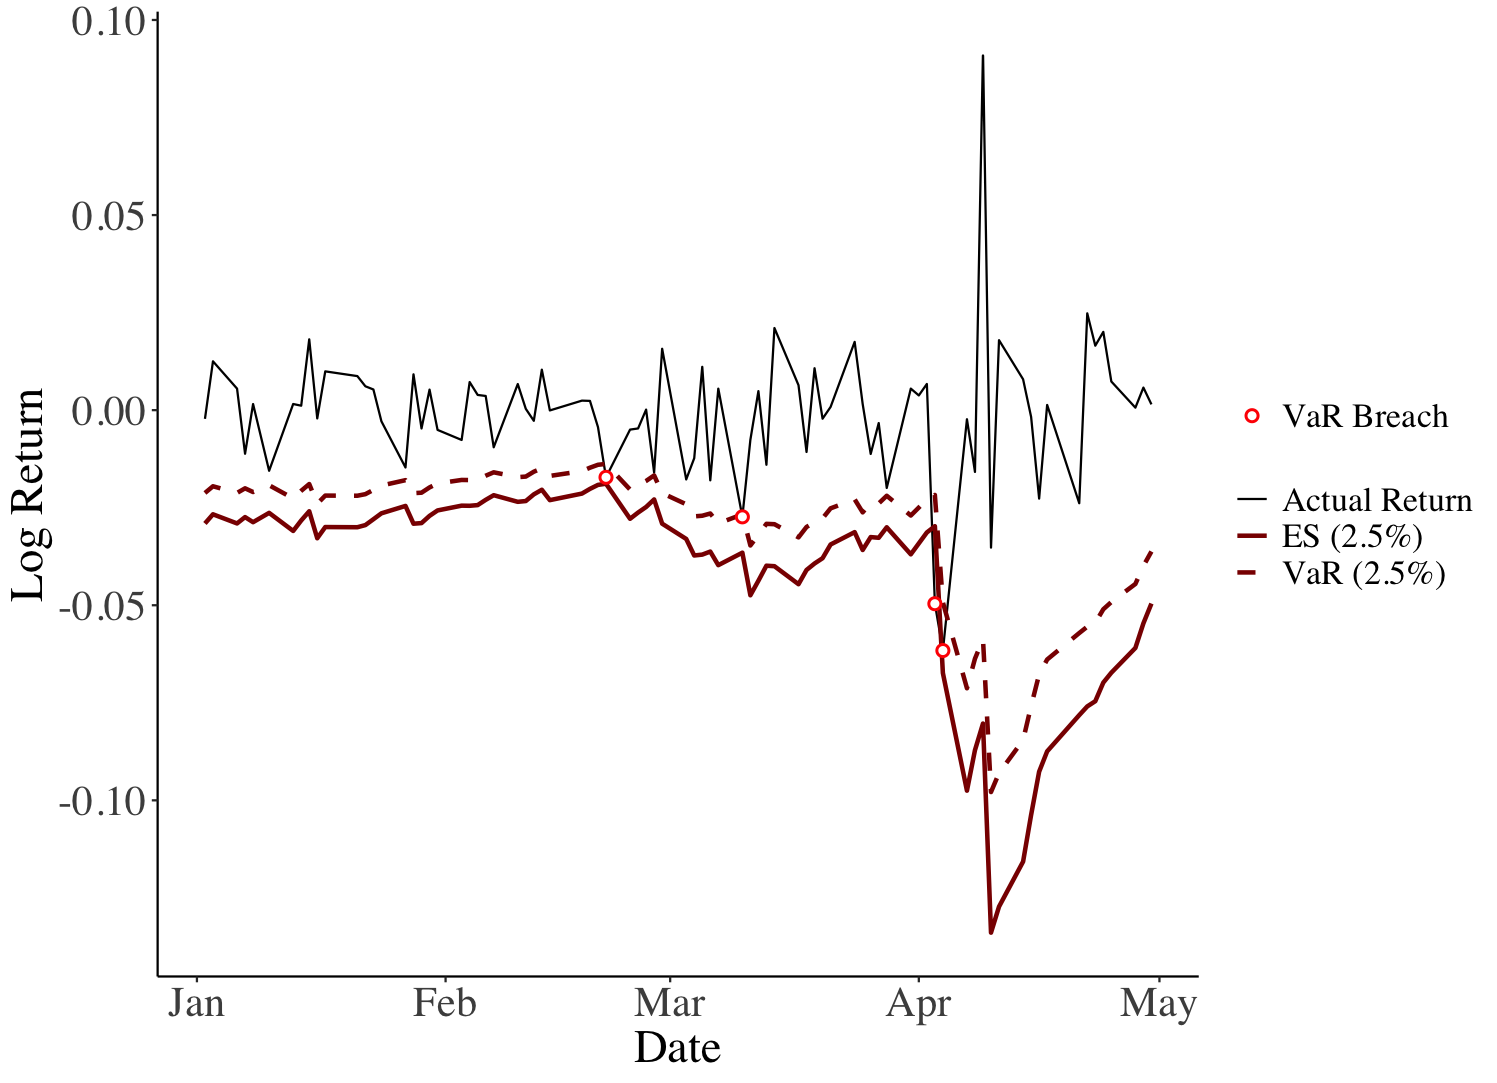
\includegraphics[scale=0.17]{../../plots/4.11.png} % Replace 
   \caption{2.5\% VaR, ES, and VaR breaches in the test period, GARCH-EVT (4 breaches observed; 2 expected).}
    \label{4.11}
\end{figure}

\begin{figure}[H]
    \centering
    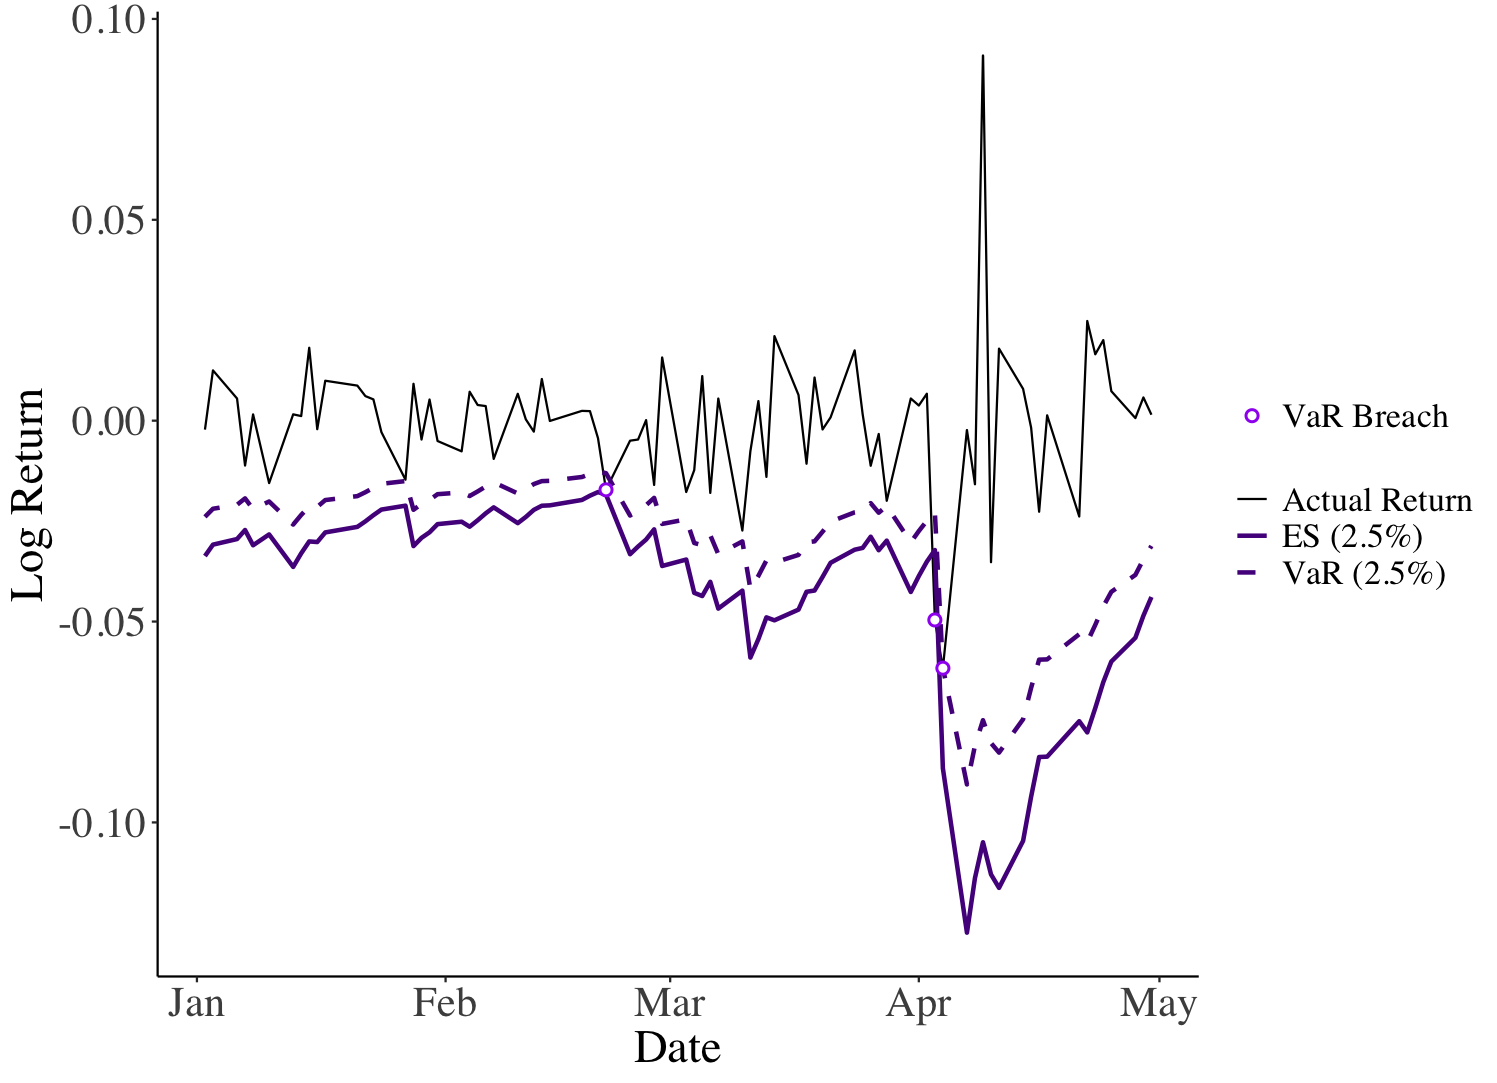
\includegraphics[scale=0.17]{../../plots/4.12.png} % Replace 
   \caption{2.5\% VaR, ES, and VaR breaches in the test period, GJR-EVT (3 breaches observed; 2 expected).}
    \label{4.12}
\end{figure}

The results of the VaR tests using the methodology of \citeA{christoffersen1998evaluating} are summarized in Table~\ref{tab:4.3}.

\begin{table}[H]
\centering
\begin{tabular}{llcc}
\toprule
\textbf{Test} & \textbf{p-value} & \textbf{GARCH-EVT} & \textbf{GJR-EVT} \\
\midrule
$LR_{\text{uc}}$   & Theoretical &  0.2138 &   0.5168 \\
                   & Simulated   & 0.188 & 0.554 \\
$LR_{\text{ind}}$  & Theoretical & 0.1582 & 0.0729 \\
                   & Simulated   & 0.03 & 0.013 \\
$LR_{\text{cc}}$   & Theoretical & 0.1706 & 0.1622 \\
                   & Simulated   & 0.217 & 0.2 \\
\bottomrule
\end{tabular}
\caption{Theoretical and simulated $p$-values for VaR testing statistics.}
\label{tab:4.3}
\end{table}

Both models offer acceptable coverage, but show weaknesses regarding the independence of VaR breaches; primarily due to the two consecutive violations at the onset of the tariff imposed by the United States. This suggests that the models respond slowly to sudden volatility increases. The GJR-EVT model provides acceptable coverage but still fails the independence test. Its comparatively better performance arises from the GJR volatility specification, which adapts more quickly to the volatility increases in the test sample (though not rapidly enough to avoid consecutive breaches), along with the more conservative tail estimation offered by the EVT approach.

Finally, as an exploratory stress-testing exercise, the four models considered (GARCH-Asyt, GJR-Asyt, GARCH-EVT, and GJR-EVT) were evaluated over the 2008 financial crisis to assess their performance from a risk management perspective. The results are presented in Figure~\ref{4.13}, where the dotted lines represent the VaR forecasts under the four models. The EVT-based models exhibit fewer VaR breaches, with the GARCH-EVT model performing best in terms of minimizing violations. Additional stress-testing methodologies and their implementation are discussed by \citeA{Christoffersen2012}.

To complement Figure~\ref{4.13}, Table~\ref{tab:4.4} disaggregates the 2008 VaR breaches into a relatively calmer January--August window and the September--December crisis window.

\begin{table}[H]
\centering
\begin{tabular}{lccc}
\toprule
\textbf{Model} & \textbf{Jan--Aug} & \textbf{Sep--Dec} & \textbf{Total} \\
\midrule
GARCH-Asyt & 9 & 7 & 16 \\
GJR-Asyt   & 8 & 5 & 13 \\
GARCH-EVT  & 4 & 5 & 9  \\
GJR-EVT    & 7 & 5 & 12 \\
\midrule
Expected   & 4.17 & 2.10 & 6.28 \\
\bottomrule
\end{tabular}
\caption{Number of 2.5\% VaR breaches by period and model during the 2008 stress test. The January--August window contains 167 trading days and the September--December window 84; the last row reports the expected number of breaches at the 2.5\% level.}
\label{tab:4.4}
\end{table}

All four specifications exceed their expected number of breaches in both sub-periods, but the deterioration is markedly sharper in September--December. The GARCH-EVT model is essentially well calibrated in the first window (4 observed against 4.17 expected) yet records more than twice the expected breaches in the second (5 against 2.10); the remaining models show an analogous widening of the gap. Since the September--December window contains roughly half as many trading days as the first, the corresponding rise in breach frequency is even more pronounced than the raw counts suggest. This pattern indicates that the four models are unable to adapt quickly enough to the abrupt regime change in September--October 2008.

Up to this point, only univariate models have been considered. While useful, such models may be insufficient for assessing the risk of a portfolio of assets, for which a multivariate framework is required. The next chapter adopts a copula-based approach to model dependence among assets and to produce multivariate forecasts. The main motivation for this choice is that copulas integrate naturally with the univariate models developed so far.

\begin{figure}[H]
    \centering
    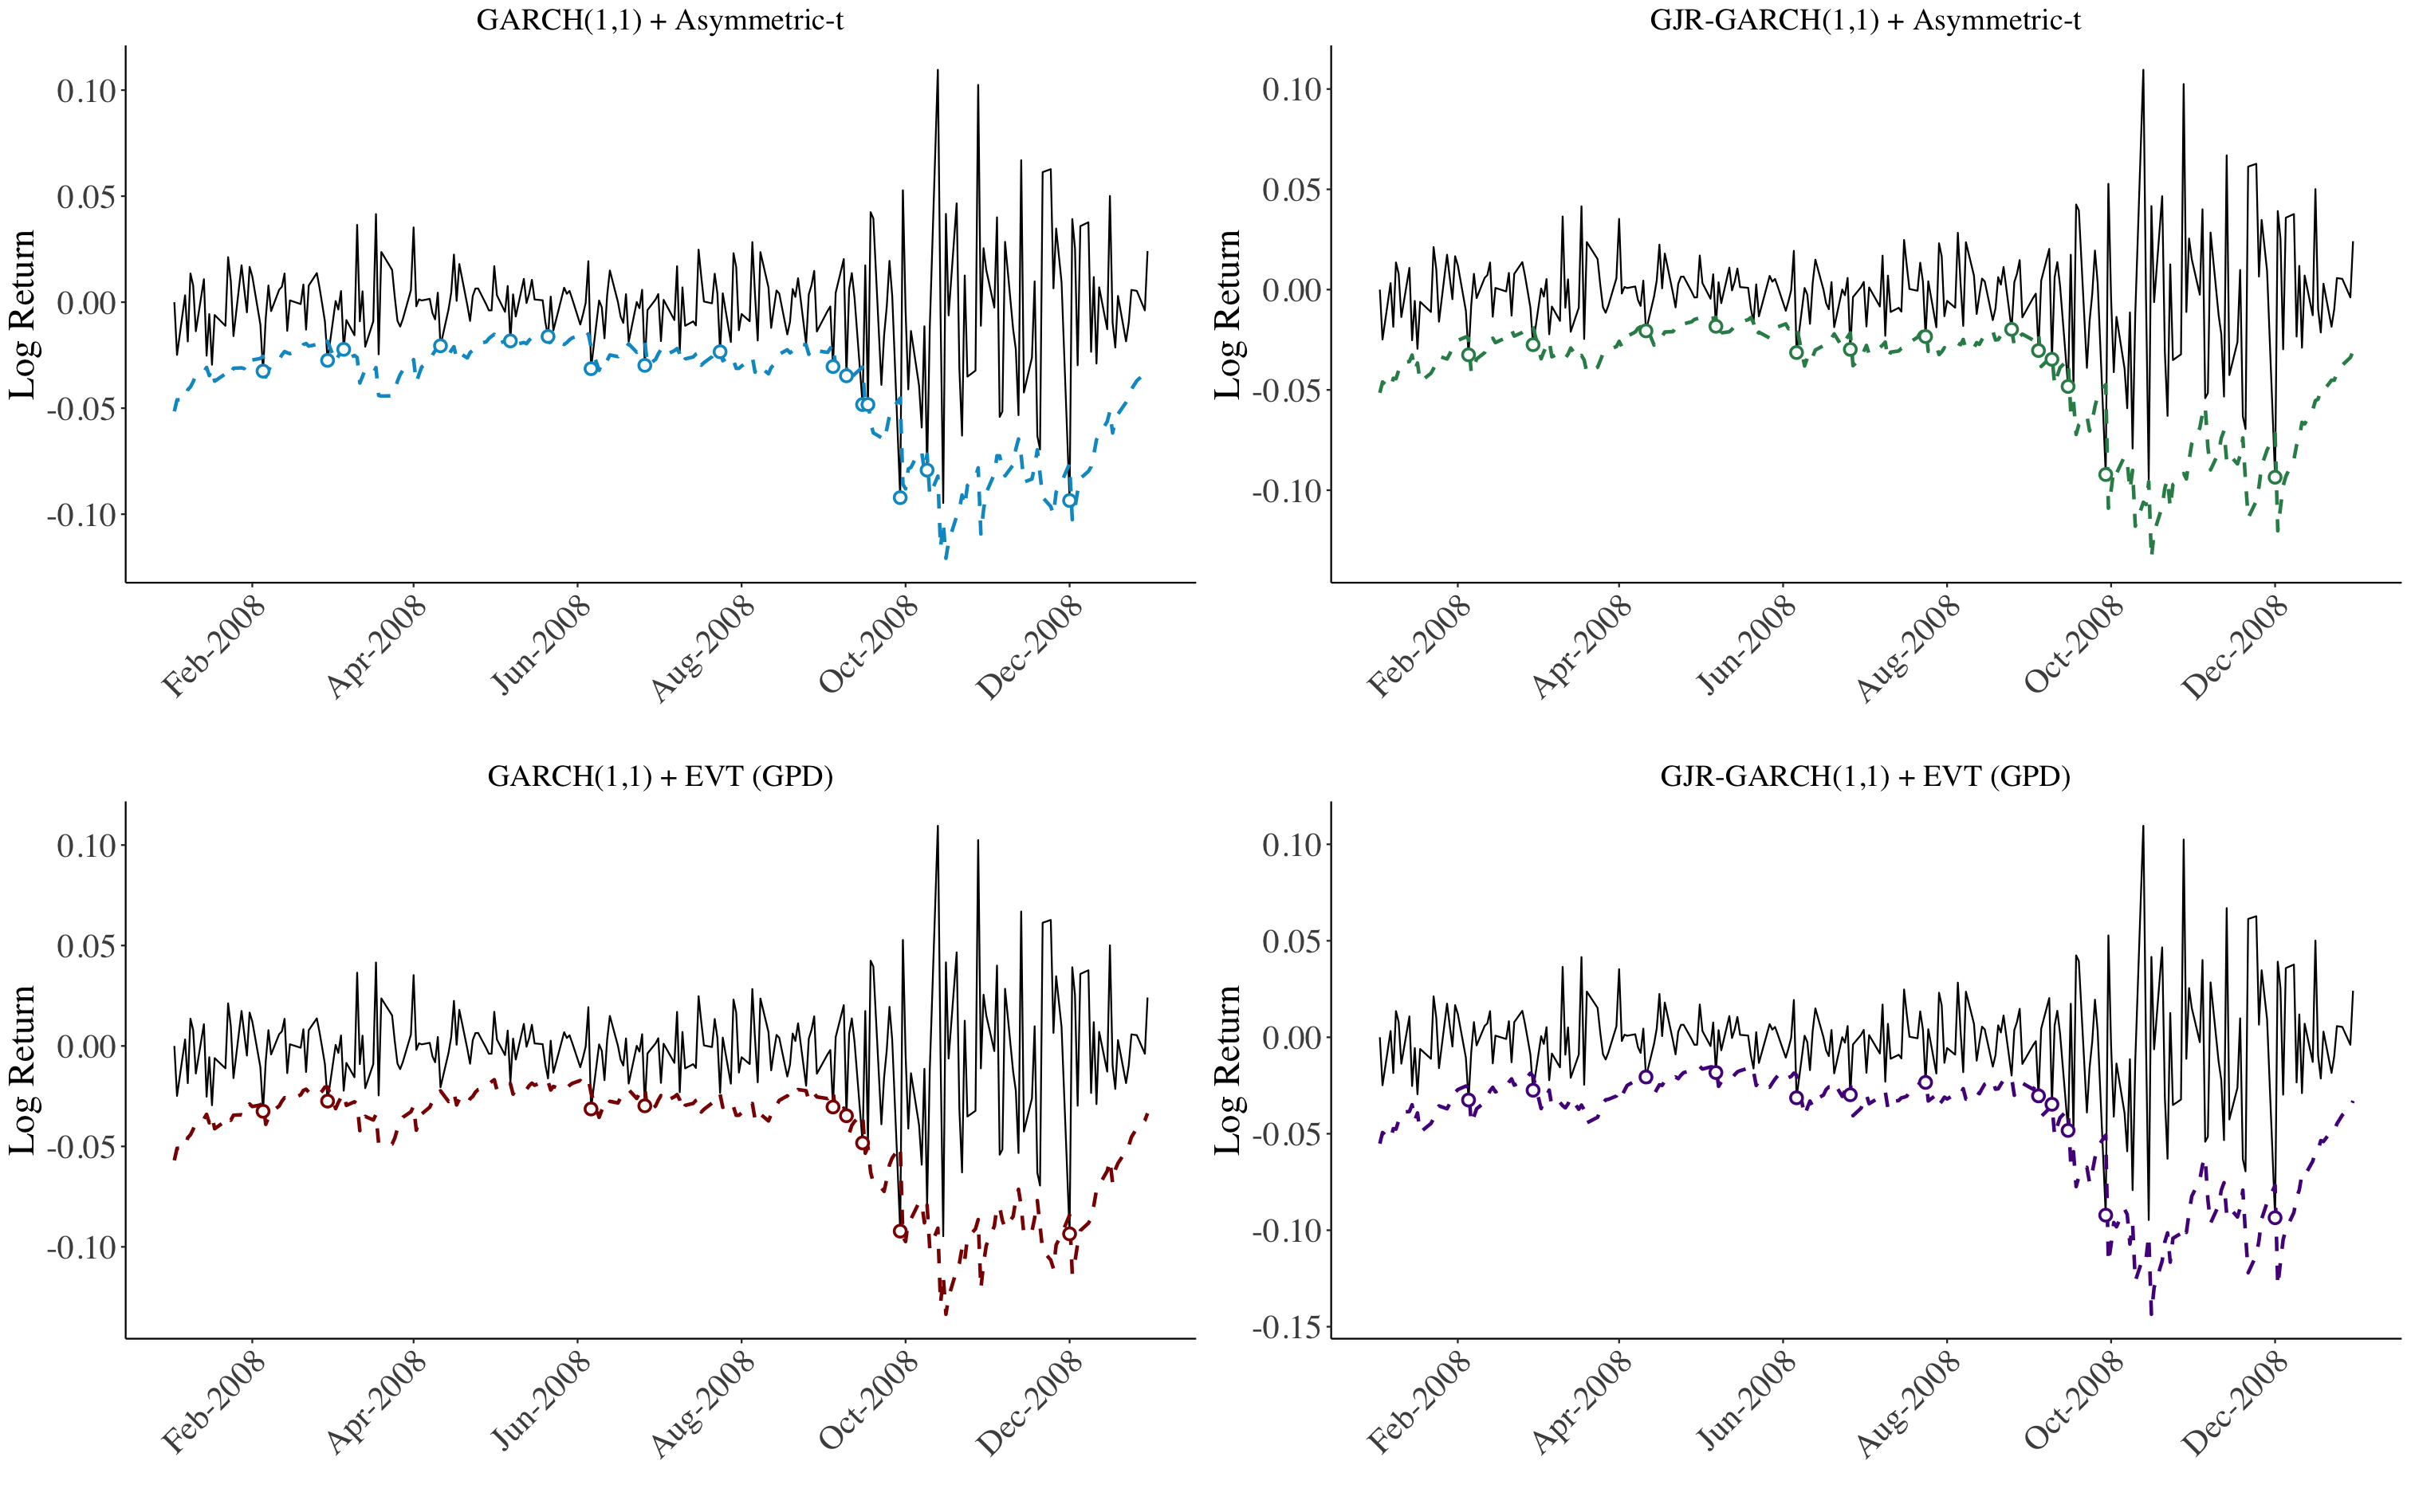
\includegraphics[scale=0.16, angle=90]{../../plots/4.13.png}
    \caption{Stress test of the models.}
    \label{4.13}
\end{figure}

\newpage